\documentclass[]{project_report}
\usepackage{graphicx}
\usepackage{hyperref}
\usepackage{tikz}




%%%%%%%%%%%%%%%%%%%%%%
%%% Input project details
\def\studentname{Edward Instance}
\def\reportyear{2024}
\def\projecttitle{Advanced Web Development}
\def\supervisorname{Christos Dexiades}
\def\degree{BSc in Computer Science}
\def\fullOrHalfUnit{Full Unit} % indicate if you are doing the project as a Full Unit or Half Unit
\def\finalOrInterim{Project Plan} % indicate if this document is your Final Report or Interim Report

\begin{document}

\maketitle

%%%%%%%%%%%%%%%%%%%%%%
%%% Declaration

\chapter*{Declaration}

This report has been prepared on the basis of my own work. Where other published and unpublished source materials have been used, these have been acknowledged.

\vskip3em

Word Count: 

\vskip3em

Student Name: \studentname

\vskip3em

Date of Submission: 

\vskip3em

Signature:

\newpage

%%%%%%%%%%%%%%%%%%%%%%
%%% Table of Contents
\tableofcontents\pdfbookmark[0]{Table of Contents}{toc}\newpage

%%%%%%%%%%%%%%%%%%%%%%
%%% Your Abstract here
\chapter*{Abstract}
\addcontentsline{toc}{chapter}{Abstract}
\newpage

%%%%%%%%%%%%%%%%%%%%%%
%%% Introduction
\chapter{Timeline}


I plan to spend the beginning of term one working on my project plan and deciding on the technologies and frameworks that I will be using. Then I will start building my application, I will be focusing on the Web and Application tier's as the data model will be defined based on them. I am hoping to have an Minimum viable product (MVP) by the end of week 8 so that I have time to test it and create my interim report by the end of week 10. After the report is submitted and I have completed the presentation I am planning to re-evaluate my plan for term 2, I am also planning to do a review in week 6 to ensure that I am on track and to help me prioritise work.


 

\section{Term 1}


\begin{center}
    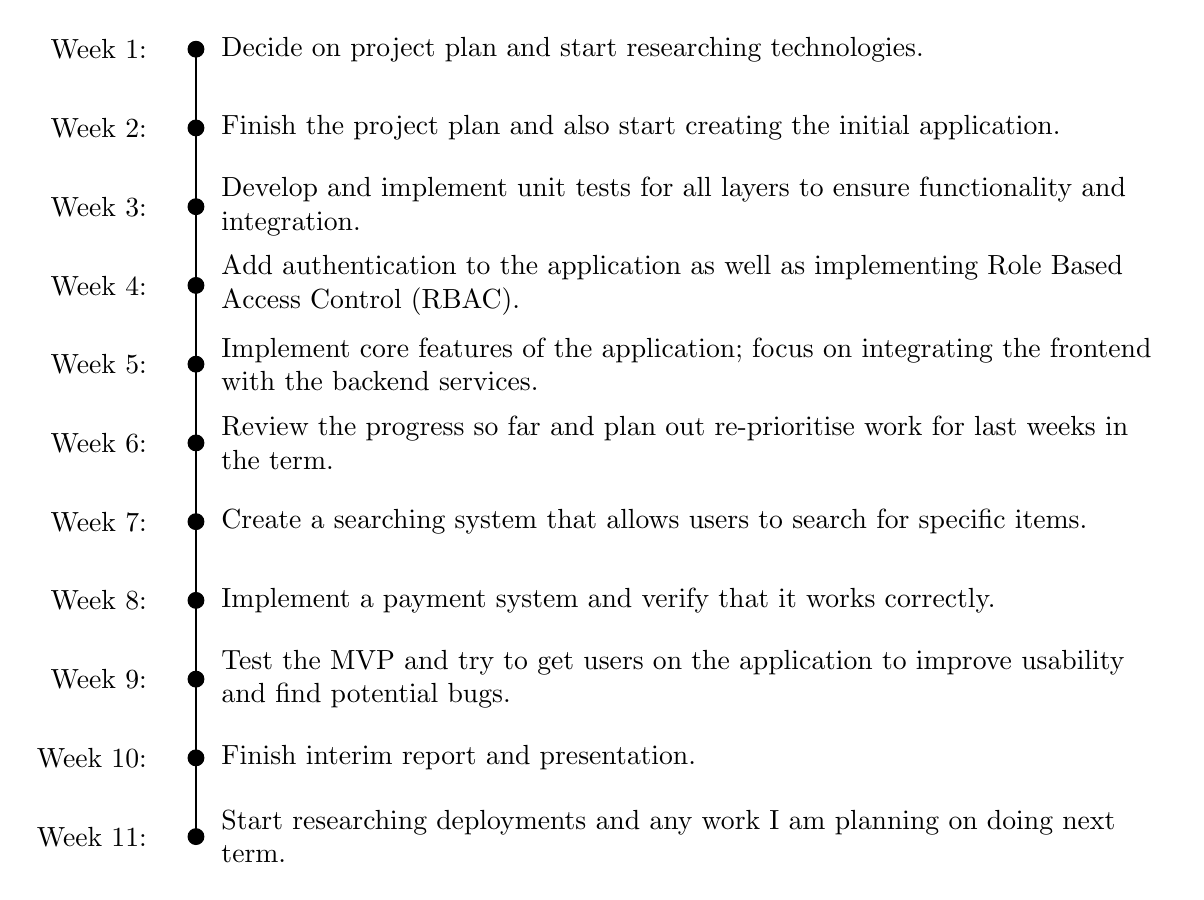
\begin{tikzpicture}[scale=1, every node/.style={scale=1}]

        \def\yshift{-1}  % Adjust the shift for better spacing
        % Draw the vertical timeline
        \draw[thick] (0,-1) -- (0,-11);  % Timeline from 0 to -10
        
        % Create the weeks and the dots for them
        \node[anchor=east] at (-0.5,\yshift) {Week 1:};
        \node[anchor=west, text width=12cm] at (0.2,\yshift) {Decide on project plan and start researching technologies.};
        \draw[fill] (0,\yshift) circle (0.1);  

        \node[anchor=east] at (-0.5,2*\yshift) {Week 2:};
        \node[anchor=west, text width=12cm] at (0.2,2*\yshift) {Finish the project plan and also start creating the initial application.};
        \draw[fill] (0,2*\yshift) circle (0.1);  

        \node[anchor=east] at (-0.5,3*\yshift) {Week 3:};
        \node[anchor=west, text width=12cm] at (0.2,3*\yshift) {Develop and implement unit tests for all layers to ensure functionality and integration.};
        \draw[fill] (0,3*\yshift) circle (0.1);  

        \node[anchor=east] at (-0.5,4*\yshift) {Week 4:};
        \node[anchor=west, text width=12cm] at (0.2,4*\yshift) {Add authentication to the application as well as implementing Role Based Access Control (RBAC).};
        \draw[fill] (0,4*\yshift) circle (0.1);  

        \node[anchor=east] at (-0.5,5*\yshift) {Week 5:};
        \node[anchor=west, text width=12cm] at (0.2,5*\yshift) {Implement core features of the application; focus on integrating the frontend with the backend services.};
        \draw[fill] (0,5*\yshift) circle (0.1);  

        \node[anchor=east] at (-0.5,6*\yshift) {Week 6:};
        \node[anchor=west, text width=12cm] at (0.2,6*\yshift) {Review the progress so far and plan out re-prioritise work for last weeks in the term.};
        \draw[fill] (0,6*\yshift) circle (0.1);  

        \node[anchor=east] at (-0.5,7*\yshift) {Week 7:};
        \node[anchor=west, text width=12cm] at (0.2,7*\yshift) {Create a searching system that allows users to search for specific items.};
        \draw[fill] (0,7*\yshift) circle (0.1);  

        \node[anchor=east] at (-0.5,8*\yshift) {Week 8:};
        \node[anchor=west, text width=12cm] at (0.2,8*\yshift) {Implement a payment system and verify that it works correctly.};
        \draw[fill] (0,8*\yshift) circle (0.1);  

        \node[anchor=east] at (-0.5,9*\yshift) {Week 9:};
        \node[anchor=west, text width=12cm] at (0.2,9*\yshift) {Test the MVP and try to get users on the application to improve usability and find potential bugs.};
        \draw[fill] (0,9*\yshift) circle (0.1);  

        \node[anchor=east] at (-0.5,10*\yshift) {Week 10:};
        \node[anchor=west, text width=12cm] at (0.2,10*\yshift) {Finish interim report and presentation.};
        \draw[fill] (0,10*\yshift) circle (0.1);  
        
        \node[anchor=east] at (-0.5,11*\yshift) {Week 11:};
        \node[anchor=west, text width=12cm] at (0.2,11*\yshift) {Start researching deployments and any work I am planning on doing next term.};
        \draw[fill] (0,11*\yshift) circle (0.1);  

    \end{tikzpicture}
\end{center}




\section{Term 2}

\chapter{Risks and Mitigation's}


%%%% ADD YOUR BIBLIOGRAPHY HERE
\newpage
\begin{thebibliography}{99}
\addcontentsline{toc}{chapter}{Bibliography}

\end{thebibliography}
\label{endpage}



\end{document}

